\documentclass[12pt,fleqn]{article}
%\usepackage {psfig,epsfig} % para incluir figuras em PostScript
\usepackage{amsfonts,amsthm,amsopn,amssymb,latexsym}
\usepackage{hyperref}
\usepackage{graphicx}
\usepackage[T1]{fontenc}
\usepackage[brazil]{babel}
\usepackage{geometry}
\usepackage{here}
\usepackage[utf8]{inputenc}
\usepackage[intlimits]{amsmath}
\usepackage{subfigure}
%alguns macros
\newcommand{\R}{\ensuremath{\mathbb{R}}}
\newcommand{\Rn}{{\ensuremath{\mathbb{R}}}^{n}}
\newcommand{\Rm}{{\ensuremath{\mathbb{R}}}^{m}}
\newcommand{\Rmn}{{\ensuremath{\mathbb{R}}}^{{m}\times{n}}}
\newcommand{\contcaption}[1]{\vspace*{-0.6\baselineskip}\begin{center}#1\end{center}\vspace*{-0.6\baselineskip}}%================================================================

% Dimensões da página
\usepackage{a4}                       % tamanho da página
\setlength{\textwidth}{16.0cm}        % largura do texto
\setlength{\textheight}{9.0in}        % tamanho do texto (sem head, etc)
\renewcommand{\baselinestretch}{1.15} % espaçamento entre linhas
\addtolength{\topmargin}{-1cm}        % espaço entre o head e a margem
\setlength{\oddsidemargin}{-0.1cm}    % espaço entre o texto e a margem
       
% Ser indulgente no preenchimento das linhas
\sloppy
 

\begin{document}
\pagestyle {empty}

% Páginas iniciais
% capa ilustrativa

\vspace*{-2cm}
{\bf
\begin{center}
{\large
\hspace*{0cm}Instituto Federal de Educação, Ciência e Tecnologia do Ceará} \\
\vspace*{0.3cm}
\hspace*{0cm}Engenharia da computação\\
\hspace*{0cm}  \\
\end{center}}
\vspace{4.0cm}
\noindent
\begin{center}
{\Large \bf Visão Computacional \\ 
\vspace*{1.0cm}
Prof. Pedro Pedrosa \\
\vspace*{1.0cm}
Relatório N$^o$ 1 - Testes com manipulação de imagens} \\[3cm]
{\Large David Paulo Magalhães Araújo}\\[6mm]

\end{center}




{\raggedleft
\begin{minipage}[t]{6.3cm}
\setlength{\baselineskip}{0.25in}

\end{minipage}\\[6cm]}
\vspace{1cm}
{\center Fortaleza \\[3mm]
Março de 2018 \\}


\newpage
%\pagestyle {empty}
%\abstract{ escrever o resumo do trabalho }

\newpage

\tableofcontents
% Numeração em romanos para páginas iniciais (sumários, listas, etc)
%\pagenumbering {roman}
\pagestyle {plain}

\setcounter{page}{0} \pagenumbering{arabic}

  
\setlength{\parindent}{0in}  %espaco entre paragrafo e margem 
% Espaçamento entre parágrafos
\parskip 5pt  
\newpage
\section{Introdução}

%comando cria itens
% \begin{itemize}
%   \item Filtro da mediana
%   \item apresentar trabalhos relacionados
%   \item apresentar motivação
%   \item apresentar objetivos
%   \item último parágrafo deve conter a organização do documento
%   \item novo item
% \end{itemize}


  \subparagraph{\normalfont Este relatório tem como objetivo principal relatar os resultados dos testes realizados com filtros 
passa alta e passa baixa, bem como os resultados dos processos de equalização e limiarização, observando as mudanças
na imagen e as razões para tais processos. A seguir, estão listados todos os processos que serão abordados nesse documento:}

\begin{itemize}
  \item Filtro da mediana
  \item Filtro da média
  \item Filtro gaussiano
  \item Filtro laplaciano
  \item Filtro sobel
  \item Filtro prewit
  \item Equalização de histograma
  \item Limiarização
  \item Multilimiarização
\end{itemize}


\section{Testes com filtros passa-baixa}

  \subparagraph{\normalfont Nessa seção abordaremos os filtros da média, mediana e gaussiano.}

  \subparagraph{\normalfont Na implementação feita em C, o filtro da mediana pode ser feito como foi mostrado anteriormente selecionando a opção 0 (carregar imagem da Lenna) e depois a opção 9 (Filtro da mediana). Já os outros filtros  passa-baixa são feitos com uma convolução (opção 6) na imagem carregada. Antes de fazer a convolução, o aplicativo solicitará por um kernel e, informando adequadamente, você consegue os filtros da média e gaussiano.}

  \subsection{Teste com filtro da mediana}

      \subparagraph{\normalfont O filtro da mediana é o único filtro passa-baixa entre os três a serem abordados que não é uma convolução de um kernel sobre uma imagem. 
      Ele consiste em em alterar os pixels da imagen para a mediana de sua vizinhança, eliminando pixels que distoem muito de seus pixels vizinhos, sendo um 
      de seus objetivos o de eliminar ruidos do tipo sal e pimenta. Um dos efeitos dele é o de deixar a imagen suavizada, sem aparentes relevos, como um tecido.}

      \begin{figure}[!htb]
      \centering
      \subfigure[Antes do filtro]{
      \hspace{-2cm} 
      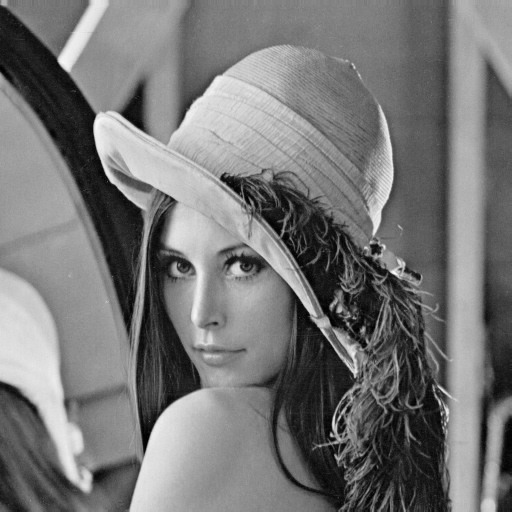
\includegraphics[height=5cm, width=5cm]{images/original.jpg}
      \label{fig:Antes do filtro}
      }\subfigure[Depois do filtro]{
      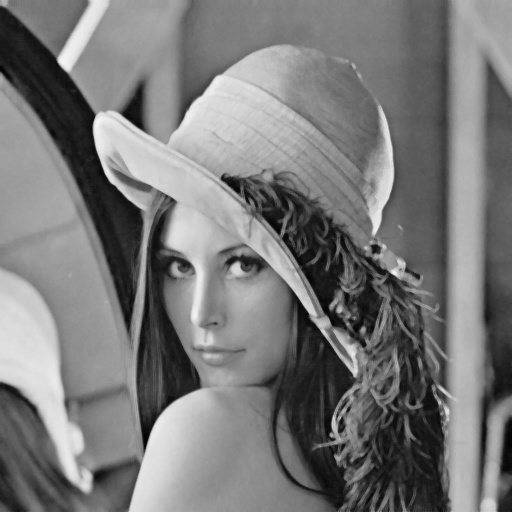
\includegraphics[height=5cm, width=5cm]{images/mediana.jpg}
      \label{fig:Depois do filtro}  
      }
      \caption{Aplicação do filtro da mediana}
      \label{fig:Resultado 1}
      \end{figure}

  \subsection{Teste com filtro da média}

      \subparagraph{\normalfont O filtro da média é feito pela média aritmética de cada pixel de uma imagen e sua vizinhança. Um dos seus principais objetivos é o de remover 
      ruídos, mas ele tem a desvantagem de não preservar tão bem as bordas ou fronteiras das imagens quando comparado ao filtro da mediana. Dado sua definição, O filtro da média 
      pode ser implementando fazendo-se uma convolução da matriz de pixels da imagem com a seguinte máscara:}

      \begin{equation*}
        \begin{bmatrix}
            1 & 1 & 1 \\
            1 & 1 & 1 \\
            1 & 1 & 1
        \end{bmatrix}
      \end{equation*}
     

      \newpage

      \begin{figure}[!htb]
      \centering
      \subfigure[Antes do filtro]{
      \hspace{-2cm} 
      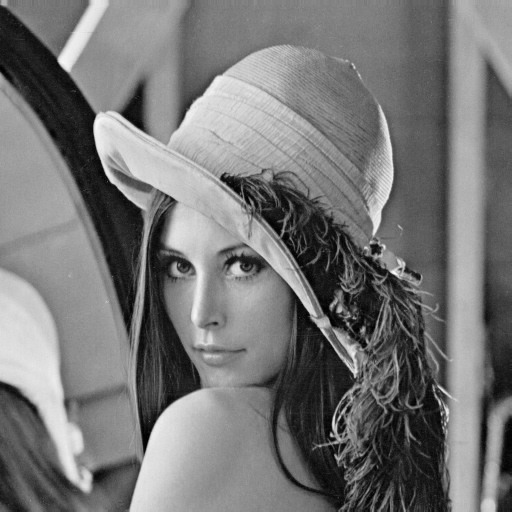
\includegraphics[height=5cm, width=5cm]{images/original.jpg}
      \label{fig:Antes do filtro}
      }\subfigure[Depois do filtro]{
      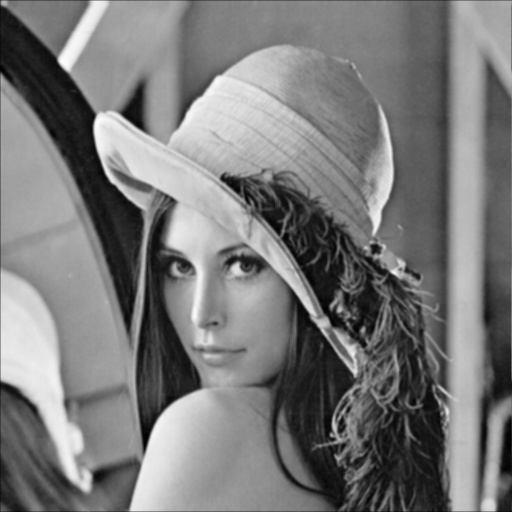
\includegraphics[height=5cm, width=5cm]{images/filtromedia.jpg}
      \label{fig:Depois do filtro}  
      }
      \caption{Aplicação do filtro da média}
      \label{fig:Resultado 1}
      \end{figure}

  \subsection{Teste com filtro gaussiano}

      \subparagraph{\normalfont O filtro gaussiano é realizado pela convolução da imagen com um kernel com valores aproximados da função gaussiana. 
      O filtro é usado para "borrar" a imagem e remover detalhes e ruídos, além de prover uma suavização mais gentil da imagem e uma preservação das bordas
      melhor do que o filtro da média. Para usar um filtro gaussiano, é necessário, primeiro, gerar um kernel com valores aproximados da função gaussiana,
      e depois fazer convolução desse com a imagem. A matrix, a seguir, é um exemplo de um kernel adequado: }


      \begin{equation*}
        \begin{bmatrix}
            1 & 4 & 7 & 4 & 1 \\
            4 & 16 & 26 & 16 & 4 \\
            7 & 26 & 41 & 26 & 7 \\
            4 & 16 & 26 & 16 & 4 \\
            1 & 4 & 7 & 4 & 1 
        \end{bmatrix}
      \end{equation*}

      \newpage

      \begin{figure}[!htb]
      \centering
      \subfigure[Antes do filtro]{
      \hspace{-2cm} 
      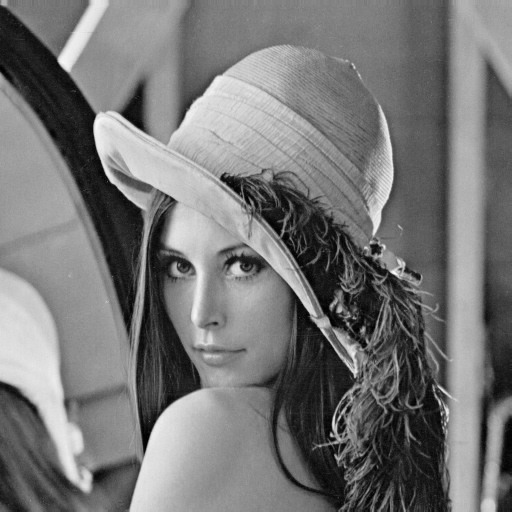
\includegraphics[height=5cm, width=5cm]{images/original.jpg}
      \label{fig:Antes do filtro}
      }\subfigure[Depois do filtro]{
      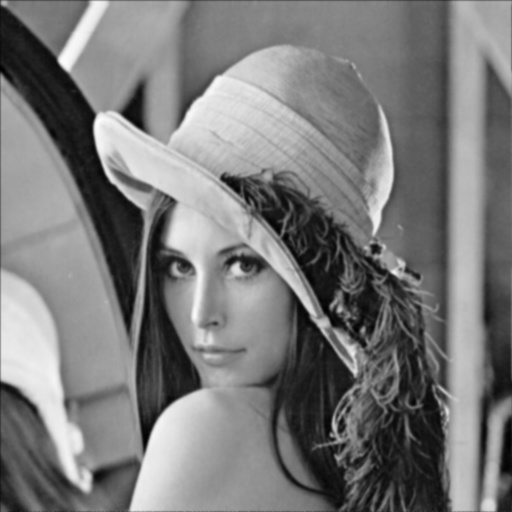
\includegraphics[height=5cm, width=5cm]{images/gaussiana.jpg}
      \label{fig:Depois do filtro}  
      }
      \caption{Aplicação do filtro gaussiano}
      \label{fig:Resultado 1}
      \end{figure}

\section{Testes com filtros passa-alta}

  \subparagraph{\normalfont Nessa seção abordaremos os filtros laplaciano, prewit e sobel.}

  \subparagraph{\normalfont Na implementação feita em C, É necessário, antes de qualquer operação, carregar uma imagem. Use a opção 0 para carregar a imagem da Lenna. 
  No caso do filtro laplaciano, após carregar a imagem, faça uma convolução (opção 6) e forneça um kernel laplaciano, e o resultado será uma imagem aplicada com o filtro laplaciano. 
  Para o prewit e o sobel, faça o seguinte passo-à-passo: }


  \begin{itemize}
    \item Carregue a imagem, caso ainda não tenha feito (Opção 0 ou Opção 1)
    \item Faça uma convoluçao (opção 6) com o kernel horizontal do filtro
    \item Guarde a imagem em memória (opção 2)
    \item Carregue a imagem original novamente (Opção 0 ou Opção 1)
    \item Faça uma convoluçao (opção 6) com o kernel vertical do filtro
    \item Selecione a opção 3
    \item Selecione a opção da raiz da soma dos quadrados (opção 2)
  \end{itemize}

  \subparagraph{\normalfont O resultado será uma imagem com o filtro sobel ou prewit, dependendo dos kernels fornecidos nas convoluções}

  \subsection{Teste com filtro laplaciano}

  \subparagraph{\normalfont A Laplaciana é uma medida isotropica 2-D da segunda derivada espacial de uma imagem. Ela destaca, na imagem, regiões em que haja rápida mudança de intensidade e é,
  portanto, frequentemente usada para detecção de bordas. a Laplaciana é frequentemente aplicada em uma imagem que foi antes suavizada com um filtro gaussiano para reduzir sua sensibilidade à ruídos.}


  \begin{equation*}
    \begin{bmatrix}
        1 & 1 & 1 \\
        1 & -8 & 1 \\
        1 & 1 & 1 
    \end{bmatrix}
  \end{equation*}

  \begin{figure}[!htb]
  \centering
  \subfigure[Antes do filtro]{
  \hspace{-2cm} 
  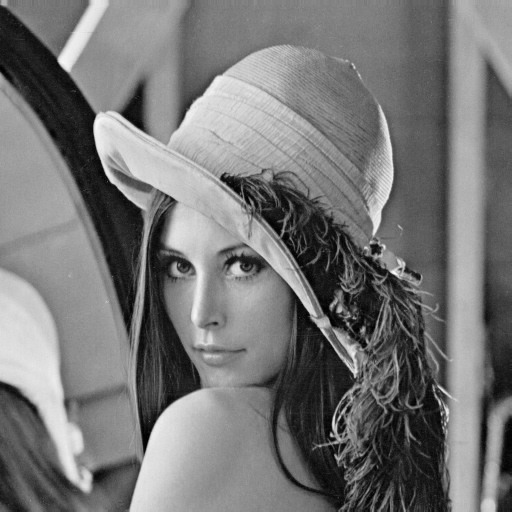
\includegraphics[height=5cm, width=5cm]{images/original.jpg}
  \label{fig:Antes do filtro}
  }\subfigure[Depois do filtro]{
  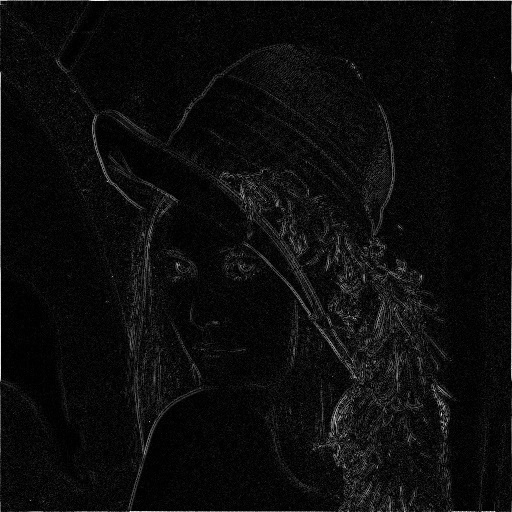
\includegraphics[height=5cm, width=5cm]{images/laplaciano.jpg} %Pode-se usar uma gaussiana antes para filtrar ruidos e melhorar a laplaciana. Laplaciana é uma gaussiana invertida?
  \label{fig:Depois do filtro}  
  }
  \caption{Aplicação do filtro laplaciano}
  \label{fig:Resultado 1}
  \end{figure}

  \newpage

  \subsection{Teste com filtro prewit}

  \subparagraph{\normalfont O filtro prewit é usado para detecção de bordas em uma imagem. Ele detecta dois tipos de bordas: horizontais e verticais. Bordas são calculadas
  através da diferença entre as intensidades dos pixels correspondentes de uma imagem. É possível somar o resultado horizontal e com o vertical e obter uma imagem destancando os dois tipos. }

  \begin{equation*}
    
    \Bigg[
      \Bigg(\begin{bmatrix}
        -1 & 0 & 1 \\
        -1 & 0 & 1 \\
        -1 & 0 & 1 
      \end{bmatrix}
      * img\Bigg)^2
    +
    
    \Bigg(\begin{bmatrix}
        -1 & -1 & -1 \\
        0 & 0 & 0 \\
        1 & 1 & 1 
    \end{bmatrix}
    * img\Bigg)^2

    \Bigg]^\frac{1}{2}
  \end{equation*}

  \begin{figure}[!htb]
  \centering
  \subfigure[Antes do filtro]{
  \hspace{-2cm} 
  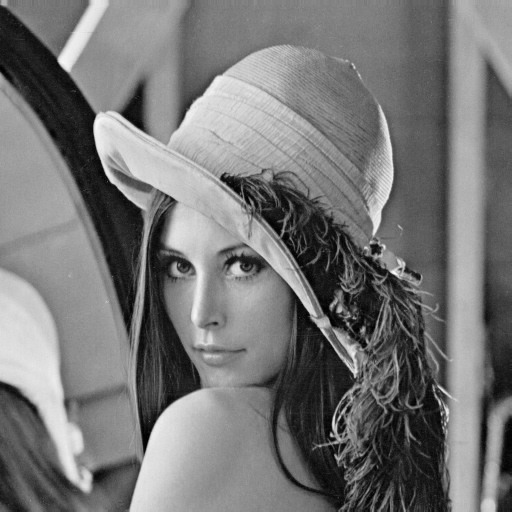
\includegraphics[height=5cm, width=5cm]{images/original.jpg}
  \label{fig:Antes do filtro}
  }\subfigure[Depois do filtro]{
  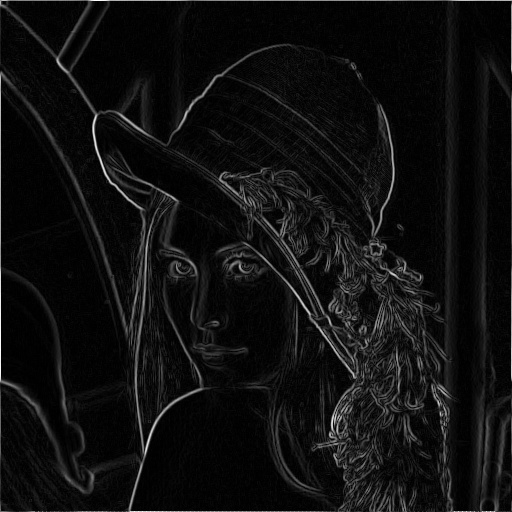
\includegraphics[height=5cm, width=5cm]{images/prewit.jpg}
  \label{fig:Depois do filtro}  
  }
  \caption{Aplicação do filtro prewit}
  \label{fig:Resultado 1}
  \end{figure}

  \subsection{Teste com filtro sobel}

  \subparagraph{\normalfont O filtro sobel é muito parecido com o filtro prewit. Ele também usa uma máscara derivadora, e é usado para detecção de bordas. 
  Como o prewit, ele também pode detectar dois tipos de bordas: horizontais e verticais. A principal diferença é que no sobel, os coeficientes da máscara
  não são fixos e podem ser ajustadas livremente, desde que não viole nenhuma propriedade de uma máscara derivadora.
  }

  \begin{equation*}
    
    \Bigg[

      \Bigg(\begin{bmatrix}
          1 & 0 & -1 \\
          2 & 0 & -2 \\
          1 & 0 & -1 
      \end{bmatrix}
      * img\Bigg)^2
      +
      
      \Bigg(\begin{bmatrix}
          1 & 2 & 1 \\
          0 & 0 & 0 \\
          -1 & -2 & -1 
      \end{bmatrix}
      * img\Bigg)^2

    \Bigg]^\frac{1}{2}
  \end{equation*}

  \begin{figure}[!htb]
  \centering
  \subfigure[Antes do filtro]{
  \hspace{-2cm} 
  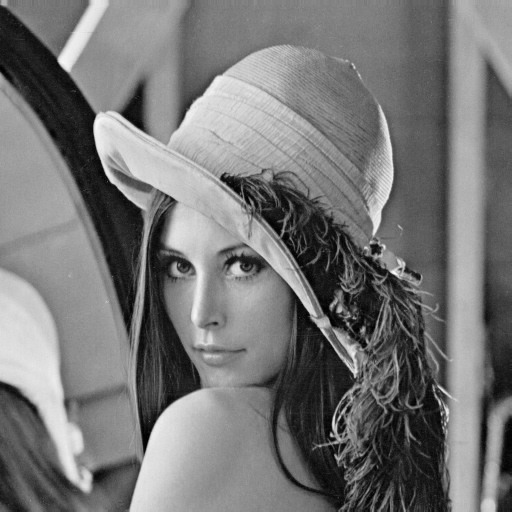
\includegraphics[height=5cm, width=5cm]{images/original.jpg}
  \label{fig:Antes do filtro}
  }\subfigure[Depois do filtro]{
  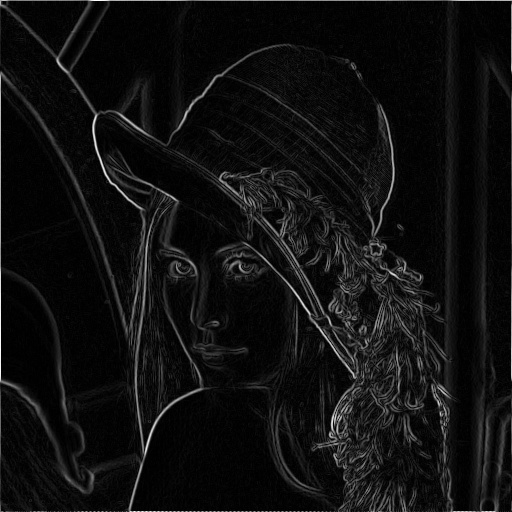
\includegraphics[height=5cm, width=5cm]{images/sobel.jpg}
  \label{fig:Depois do filtro}  
  }
  \caption{Aplicação do filtro sobel}
  \label{fig:Resultado 1}
  \end{figure}

\newpage

\section{Testes com equalização}

  \subparagraph{\normalfont Nessa seção abordaremos os efeitos da equalização, tanto para o histograma da imagem quanto pra imagem em si.}
  \subparagraph{\normalfont A equalização consiste em redistribuir a frequencia em que certas tonalidades de pixels aparecem na imagem, com o intuito de deixá-los o mais próximo possível.
  O efeito implicado da equalização é o aumento do contraste da imagem, devido a uma distribuição mais homogênea das cores ou tonalidades de cinza. O efeito no histograma é 
  o de um gráfico mais suavizado e com menos oscilações do que o original.}

  \subparagraph{\normalfont Para executar uma equalização de imagem na implementação em C, primeiro carregue uma imagem (opção 0 ou opção 1) e depois selecione equalização (opção 7)}

  \begin{figure}[!htb]
  \centering
  \subfigure[Antes]{
  \hspace{-2cm} 
  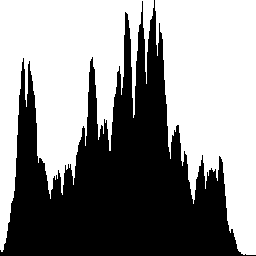
\includegraphics[height=5cm, width=5cm]{images/histograma_original.png}
  \label{fig:Antes do filtro}
  }\subfigure[Depois]{
  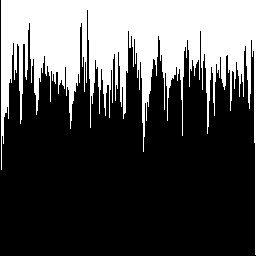
\includegraphics[height=5cm, width=5cm]{images/histograma_equalizado.png}
  \label{fig:Depois do filtro}  
  }
  \caption{Efeito da equalização no histograma da imagem}
  \label{fig:Resultado 1}
  \end{figure}

  \begin{figure}[!htb]
  \centering
  \subfigure[Antes]{
  \hspace{-2cm} 
  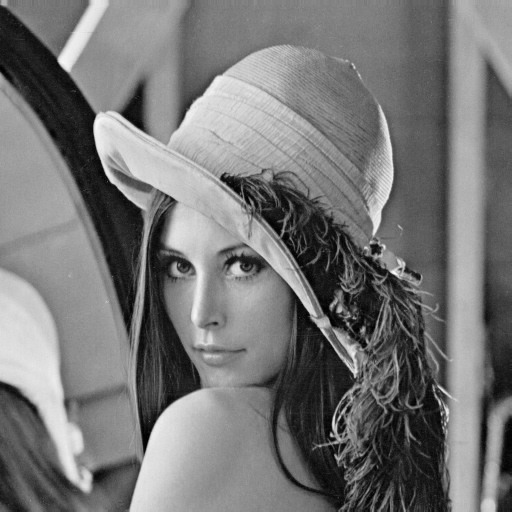
\includegraphics[height=5cm, width=5cm]{images/original.jpg}
  \label{fig:Antes do filtro}
  }\subfigure[Depois]{
  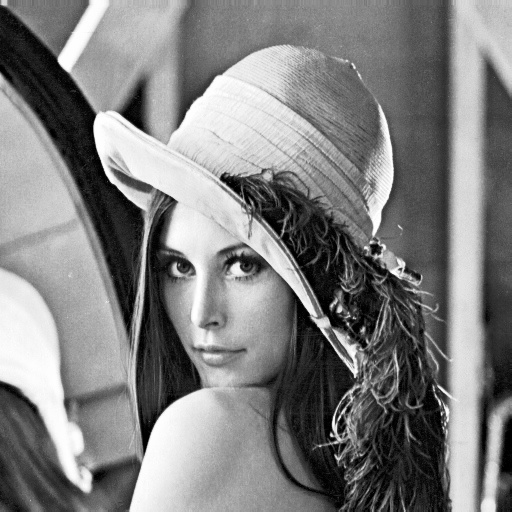
\includegraphics[height=5cm, width=5cm]{images/equalizado.jpg}
  \label{fig:Depois do filtro}  
  }
  \caption{Efeito da equalização na imagem}
  \label{fig:Resultado 1}
  \end{figure}


\section{Testes com limiarização e multilimiarização}
  \subparagraph{\normalfont Nessa seção abordaremos os efeitos da limiarização e da multilimiarização na imagem}
  \subparagraph{\normalfont A limiarização consiste em transformar todas as tonalidades da imagem para branco ou preto, tomando como referência um pivô escolhido arbitrariamente. 
  Ou seja, escolhido uma tonalidade central, todas as tonalidades menores do que essa serão transformadas em preto, e todas que forem iguais ou maiores à ela, se tornarão brancas.
  A Multilimiarização, por sua vez, divide todas as tonalidades em 3 ou mais, sendo elas branco, preto e outra(s) tonalidade(s) intermediária(s).
  }

  \newpage

  \subparagraph{\normalfont Para executar uma limiarização ou multilimiarização de imagem na implementação em C, primeiro carregue uma imagem (opção 0 ou opção 1) 
  depois selecione limiarização (opção 8). Informe a quantidade de limiares, sendo 1 para limiarização e 2 ou mais para uma multilimiarização, depois disso será
  solicitado um pivô (ou mais) para realizar o processo escolhido.}

  \begin{figure}[!htb]
  \centering
  \subfigure[Antes]{
  \hspace{-2cm} 
  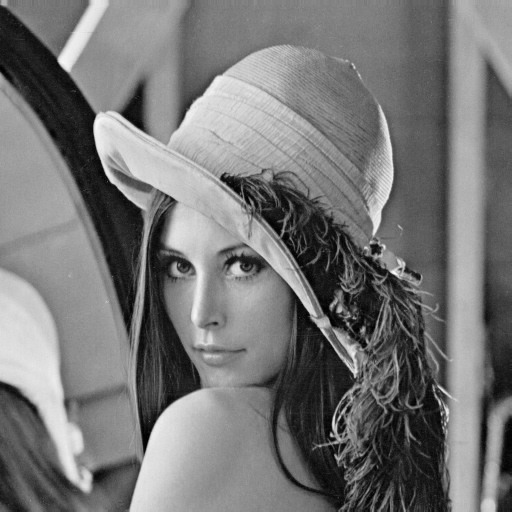
\includegraphics[height=5cm, width=5cm]{images/original.jpg}
  \label{fig:Antes do filtro}
  }\subfigure[Depois]{
  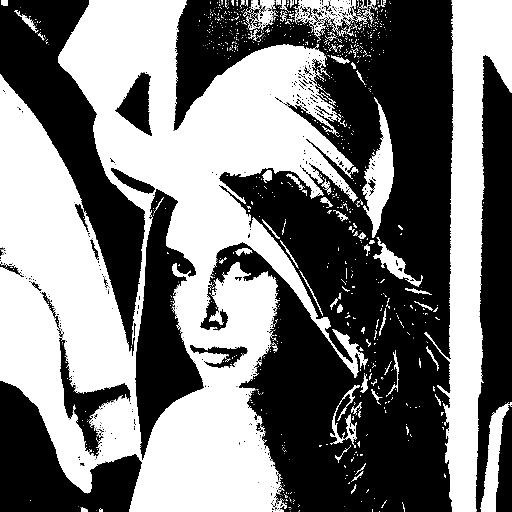
\includegraphics[height=5cm, width=5cm]{images/limiarizacao.jpg}
  \label{fig:Depois do filtro}  
  }
  \caption{Efeito da limiarização na imagem}
  \label{fig:Resultado 1}
  \end{figure}

  \begin{figure}[!htb]
  \centering
  \subfigure[Antes]{
  \hspace{-2cm} 
  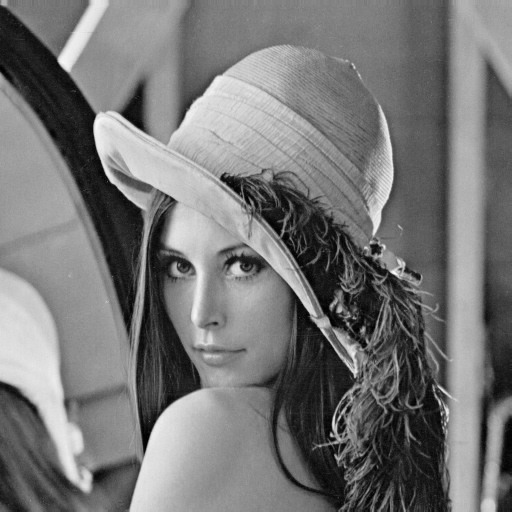
\includegraphics[height=5cm, width=5cm]{images/original.jpg}
  \label{fig:Antes}
  }\subfigure[Depois]{
  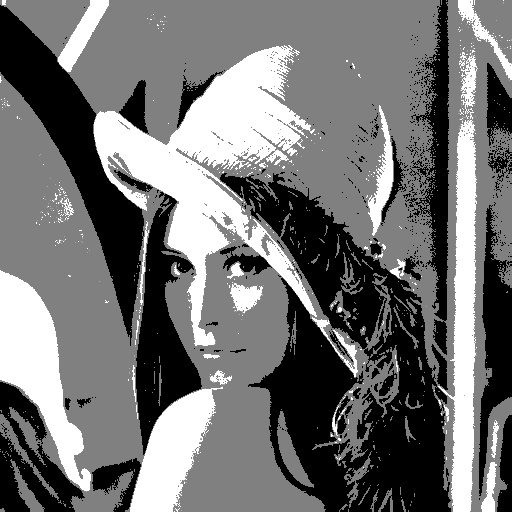
\includegraphics[height=5cm, width=5cm]{images/multilimiarizacao.jpg}
  \label{fig:Depois }  
  }
  \caption{Efeito da multilimiarização na imagem}
  \label{fig:Resultado 1}
  \end{figure}

\section{Resumo Geral}

  \subparagraph{\normalfont Esse documento faz um breve relatório dos resultados obtidos pela implementação em C dos filtros e processos de manipulação de imagem abordados por ele. 
  No decorrer do relatório, é possível notar que os resultados obtidos estão dentro do esperado para os testes realizados, vinculando teoria e prática como eram
  os objetivos do documento.}

  \subparagraph{\normalfont O documento ensina, também, como usar a implementação feita em C para verificar os testes que foram feitos e comparar com os
  resultados obtidos.}

\section{Referências Bibliográficas}

Filtro da mediana (Em inglês): \\
  \href{https://homepages.inf.ed.ac.uk/rbf/HIPR2/median.htm}{\textit{https://homepages.inf.ed.ac.uk/rbf/HIPR2/median.htm}} \\

Filtro gaussiano (Em inglês): \\
  \href{https://homepages.inf.ed.ac.uk/rbf/HIPR2/gsmooth.htm}{\textit{https://homepages.inf.ed.ac.uk/rbf/HIPR2/gsmooth.htm}} \\

Filtro laplaciano (Em inglês): \\
  \href{https://homepages.inf.ed.ac.uk/rbf/HIPR2/log.htm}{\textit{https://homepages.inf.ed.ac.uk/rbf/HIPR2/log.htm}} \\ 

Filtro sobel (Em inglês): \\
  \href{https://www.tutorialspoint.com/dip/sobel_operator.htm}{\textit{https://www.tutorialspoint.com/dip/sobel_operator.htm}} \\ 

Aula 3 da cadeira de visão computacional do IFCE: \\
  \href{https://www.dropbox.com/s/yarq1zlgv5b9zwp/VC%20-%20Aula%203.pdf?dl=0}{\textit{https://www.dropbox.com/s/yarq1zlgv5b9zwp/VC\%20-\%20Aula\%203.pdf?dl=0}} \\

Aula 4 da cadeira de visão computacional do IFCE: \\
  \href{https://www.dropbox.com/s/y50pfpwl6ueby0n/VC%20-%20Aula%204.pdf?dl=0}{\textit{https://www.dropbox.com/s/y50pfpwl6ueby0n/VC\%20-\%20Aula\%204.pdf?dl=0}} \\


\bibliographystyle{unsrt}
\bibliography{bibliografia}





% %\label{sec:tab}
% \begin{table}[htb]
% \caption{Tabela de Exemplo...}
% \label{tab:Ex1}
% \begin{center}
% 		\begin{tabular}{@{}lcccccc@{}}\hline
% 		  & IRIS (binário) & IRIS & Coluna & Dermatologia &  OR \\\hline \hline
% 		Número de Padrões   & 150 & 150 & 310 & 358 & 80 \\\hline
% 		Número de Atributos & 4   & 4   & 6   & 34  & 2 \\\hline
% 		Número de Classes   & 2   & 3   & 3   & 6   & 2 \\\hline
% 		\end{tabular}
% \end{center}
% \end{table}


% \begin{equation}
%   \label{eq:ex1}
%   A=B+C
% \end{equation}

% \begin{equation}
%   \label{eq:ex2}
%   \sigma = \mu + \delta
% \end{equation}

% Para citar trechos das fórmulas no texto basta colocar o que quer citar entre cifrão ``\$'' (ver o código do latex para citar o $\sigma$, $\mu$ e $\delta$ sem estar dentro de equações). 

% Para citar equações, tabelas e figuras, deve-se usar $\ $$\ $ref e colocar a label que identifica cada um destes elementos. Por exemplo, Figura \ref{fig:FigExMulti1}, Tabela \ref{tab:Ex1}, Equações \ref{eq:ex1} e \ref{eq:ex2}. 

% \begin{figure}[!htb]
% \centering
% \subfigure[Íris 2-Classes]{
% \hspace{-2cm} 
% \includegraphics[scale=0.3]{fig/fig1a.png}
% \label{fig:FigExMulti1a}
% }\subfigure[Íris 3-Classes]{
% \includegraphics[scale=0.3]{fig/fig1b.png}
% \label{fig:FigExMulti1b}  
% }
% \caption{Exemplo de multiplas figuras 1.}
% \label{fig:FigExMulti1}
% \end{figure}

% \begin{figure}[!htb]
%    \centering
%    \subfigure[]{\label{fig:FigExMulti2a}\includegraphics[width=0.4\hsize]{fig/fig1a.png}}
%    \hspace{0.005\hsize}
%    \subfigure[]{\label{fig:FigExMulti2b}\includegraphics[width=0.4\hsize]{fig/fig1b.png}}
%    \caption{Exemplo 2 de figuras multiplas.}
%    \label{ex3dDetails}
% \end{figure}

% \begin{figure}[!hbt]
% \begin{center}
% \includegraphics[scale=0.2]{fig/fig1a.png}
% \end{center}
% \caption{\label{ExfigIndividual}\hspace{-0.4em} Exemplo de como adicionar figuras individuais.}
% \end{figure}

% %\clearpage

% \section{Sites que ajudam na escrita com Latex} 

% Nas subseções à seguir estão sites para ajudar a fazer equações e tabelas.

% \subsection{Sites para fazer Equações}

% Site 1:

% \href{http://www.codecogs.com/latex/eqneditor.php?lang=pt-br}{\textit{http://www.codecogs.com/latex/eqneditor.php?lang=pt-br}}

% Site 2:

% \href{http://www.hostmath.com}{\textit{http://www.hostmath.com}}

% \subsection{Sites para fazer Tabelas}

% Site 1:

% \href{http://www.tablesgenerator.com}{\textit{http://www.tablesgenerator.com}}

% Site 2: 

% \href{http://truben.no/table/}{\textit{http://truben.no/table/}}

% Site 3:

% \href{http://truben.no/table/old/}{\textit{http://truben.no/table/old/}}

% \section{Editores de Latex}

% O mais usado editor de latex on line e gratuito é o Overleaf (\href{https://www.overleaf.com}{\textit{https://www.overleaf.com}}). Basta criar um novo projeto e fazer upload da pasta do projeto zipado, que o projeto é carregado e habilitado para edição online na plataforma. Existe outros Editores de texto em latex, mas o overleaf facilita o uso por ser gratuito e on line.

% \section{Referências Bibliográficas}

%  As referências são necessárias para embasar o conteúdo que está sendo discutido, principalmente detalhes técnicos que estão em destaque. As referências são inseridas usando o comando $\ $cite, e já gera a lista de referências no fim seguindo o modelo (template) usado. Abaixo seguem alguns exemplos (veja o código do arquivo *tex).
 
%  Quando eu quero resumir ou destacar algo de algum artigo, livro eu adiciono tal citação, como por exemplo \cite{Adler89} (veja o código do arquivo *tex).
 

% \section{Resumo Geral}

% Após apresentar os cálculos para cada simulação, apresente as respectivas simulações, inclusive com todas as variações possíveis, discutindo e/ou apresentando alguma conclusão sobre as simulações relacionando com a teoria. 

% \bibliographystyle{unsrt}
% \bibliography{bibliografia}

\end{document} %finaliza o documento
